\section{Operating Modes}

The UART module supports standard asynchronous serial communication via TX (transmit) and RX (receive) lines. Both transmitter and receiver can operate concurrently for full-duplex communication. Key features:

\begin{figure}[H]
    \centering
    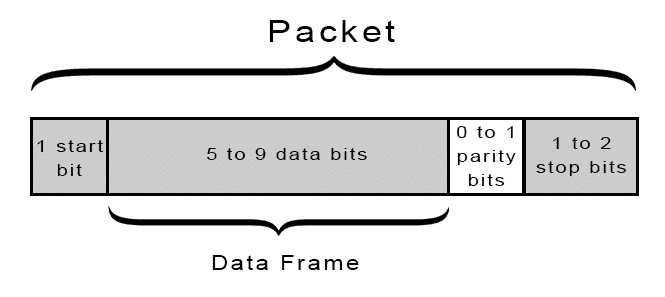
\includegraphics[width=0.85\textwidth]{images/frame_format.png}
    \caption{Frame Formats}
    \label{fig:frame_formats}
  \end{figure}

  
\begin{itemize}
  \item \textbf{Baud Rate Configuration}: Programmable via \texttt{clocksPerBitDb} register for fine-grained timing control.
  \item \textbf{Data Bits}: The number of data bits transmitted/received can be adjusted up to \texttt{maxOutputBits}.
  \item \textbf{Optional Parity}: Parity can be enabled or disabled and can be set to odd or even, controlled at runtime.
  \item \textbf{FIFO Buffers}: Internal TX and RX FIFOs provide buffering to decouple software and hardware rates.
  \item \textbf{Error Detection}: Overrun errors, underflow/overflow of FIFO, parity errors, start/stop bit errors are flagged in dedicated status registers.
\end{itemize}

\subsection{Transmitter}
\begin{itemize}
  \item Data to be sent is written to a TX FIFO, from which the transmitter fetches bytes automatically.
  \item A \textbf{start} bit (\texttt{0}) is transmitted first, followed by data bits (least significant bit first), an optional parity bit, and one or more stop bits (\texttt{1}).
  \item Transmission can begin automatically when data is available in the FIFO and the transmitter is in the \texttt{Idle} state.
  \item Overflows are flagged if software attempts to write to a full TX FIFO.
\end{itemize}

\subsection{Receiver}
\begin{itemize}
  \item The RX input line is sampled at a programmable rate defined by \texttt{clocksPerBitDb}.
  \item When a \textbf{start} bit (\texttt{0}) is detected, the receiver state machine starts shifting in data bits, optionally checking parity, and then the stop bit(s).
  \item Received bytes are pushed into the RX FIFO for software retrieval.
  \item Errors are flagged for framing errors (bad start/stop bit), parity errors, and FIFO overflow if the RX FIFO is full.
\end{itemize}

\subsection{FIFO Handling}
\begin{itemize}
  \item The TX FIFO and RX FIFO each have a configurable depth. Their status (\texttt{empty}, \texttt{full}, \texttt{halfFull}, and \texttt{count}) are exposed via registers for software polling.
  \item Software can poll \texttt{txFifoEmpty} to know if the transmitter has finished sending all data.
  \item The RX FIFO is read by polling \texttt{rxDataAvailable} or by reading the \texttt{rxFifoEmpty} status.
\end{itemize}
